%----------------------------------------------------------
%
\documentclass[xcolor=dvipsnames]{beamer}%

\mode<presentation> {
  \usetheme{CambridgeUS}
  \usefonttheme[onlymath]{serif}
  \setbeamercovered{transparent}
}

\usepackage{hyperref}

\hypersetup{colorlinks,linkcolor=,urlcolor=blue}
\usepackage{minted}
\usepackage{multicol}
%\usepackage{utf-8}

\setbeamertemplate{itemize item}{\raisebox{0.25ex}{\small\textbullet}}
\setbeamertemplate{itemize subitem}{\raisebox{0.25ex}{\scriptsize\textbullet}}
\graphicspath{{figures/}}
\logo{\resizebox{10mm}{!}{
\includegraphics{fer_logo.jpg}}}
\setbeamersize{text margin left=15pt, text margin right=20pt} 
\setlength{\leftmarginii}{10pt}
\setbeamertemplate{enumerate item}{
    \raisebox{-1.7pt}{\scalebox{2.1}{\textbullet}\hskip-14.3pt}
    \hbox to2ex{%
      \hfil
      \usebeamercolor[bg]{item projected}
      \color{fg}
      \raisebox{1.7pt}{\scalebox{0.65}{\insertenumlabel}}%
      \hfil}
    \hskip-5pt%
}
\setbeamertemplate{section in toc}{
  \leavevmode\leftskip=3ex%
  \llap{%
    \usebeamerfont*{section number projected}%
    \usebeamercolor{section number projected}%
    \begin{pgfpicture}{-1ex}{-0.3ex}{1ex}{2ex}
      \color{bg}
      \pgfpathcircle{\pgfpoint{0pt}{.75ex}}{1.7ex}
      \pgfusepath{fill}
      \pgftext[base]{\color{fg}\inserttocsectionnumber}
    \end{pgfpicture}\kern2.25ex%
  }%
  \inserttocsection\par}
\setbeamertemplate{subsection in toc}
  {\leavevmode\leftskip=2em$\bullet$\hskip1em\inserttocsubsection\par}

%------------------------------------------------------------------

%%% --------------------------------------------------------------
\title[git basics]
{LARICS git tutorial: basics}

\author[Mikli\'{c}, Or\v{s}uli\'{c}]{Damjan Mikli\'{c}, Juraj Or\v{s}uli\'{c}}

\institute[LARICS]{LARICS Lab\\FER, University of Zagreb}

\date[]{April 2017}

%\AtBeginSection[]
%{
%  \begin{frame}<beamer>{Outline}
%    \tableofcontents[currentsection]
%  \end{frame}
%}

\begin{document}
% ================================================================

\begin{frame}
	\titlepage
\end{frame}

% ----------------------------------------------------------------
\section*{Outline}
\begin {frame}
	\tableofcontents
\end{frame}


% =============================================================================

\section{Preparation}

\begin{frame}[fragile]

\frametitle{A note on notation}
	
Throughout the presentation, the following notation applies:

\begin{itemize}
	\item Commands that you are supposed to type are displayed in \texttt{monospace font} preceded by a \texttt{>} symbol, such as
	\begin{minted}{console}
> git --help
	\end{minted}
	\item The \texttt{>} symbol only indicates the command prompt.\\ \textit{Do not} type it in.
	\item When the command is too long to fit on one line, the line break will be marked with a backslash (\textbackslash), which you do not need to type.
	\item Text that you need to replace is given \texttt{<inside angle brackets>}, e.g.,
	\begin{minted}{console}
> cd /home/<your username>
	\end{minted}
	When typing the command with your replaced text,\\omit the brackets.
\end{itemize}

\end{frame}

% -----------------------------------------------------------------------------

\begin{frame}[fragile]

\frametitle{Preparing for the tutorial}
	
\begin{itemize}
	\item  Open a \href{https://github.com/join?source=header-home}{GitHub account} and set up an SSH key for passwordless login according to \href{https://help.github.com/articles/adding-a-new-ssh-key-to-your-github-account/}{these instructions}
	\item Install the \href{https://atom.io/}{Atom} text editor
	\item Install the git command-line client and GUI tools
	\begin{minted}{console}
> sudo apt install git git-gui gitg
	\end{minted}
	\item Tell git who you are, and which editor to use:
	\begin{minted}{console}
> git config --global user.name "<Your Name>"
> git config --global user.email <youremail@fer.hr>
> git config --global core.editor "atom --wait"
	\end{minted}
	\item The code example in the exercise will be available in C++ and Python. If you will be using C++, install the build tools:
	\begin{minted}{console}
> sudo apt install build-essential cmake
	\end{minted}
\end{itemize}

\end{frame}

% -----------------------------------------------------------------------------

\begin{frame}

\frametitle{Tutorial organization}
	
\begin{itemize}
	\item Work in pairs
	\item Pair up with someone using the same programming language (C++ or Python)
\end{itemize}
	
\end{frame}

% -----------------------------------------------------------------------------


% =============================================================================

\section{The basic basics}

\begin{frame}
	\frametitle{About git\footnote{\emph{git} means "unpleasant person" in British slang. Linus: "I'm an egotistical bastard, and I name all my projects after myself."}}
	
	\begin{itemize}
		\item A \emph{distributed} version control system (VCS) 
		\item Developed in 2005 by Linus Torvalds to support Linux kernel development
		\item Git was never meant to be used directly :)
		\item Very powerful and very complex
		\item Supports different workflows
		\item We'll be using the GitHub workflow (more or less)	
	\end{itemize}
	
\end{frame}

% -----------------------------------------------------------------------------

\begin{frame}
	\frametitle{VCS requirements}
	
	\begin{block}{Basic requirements}
	\begin{itemize}
		\item Keep track of changes to our code
		\item Facilitate collaboration
	\end{itemize}
	\end{block}
	
	\begin{block}{Additional requirements}
	\begin{itemize}
		\item Work offline
		\item Support a distributed workflow
		\item Compatibility with existing protocol (e.g. ssh, http)
		\item Cryptographic authentication of history
		\item Efficiency
	\end{itemize}
	\end{block}
\end{frame}

% -----------------------------------------------------------------------------

\begin{frame}[fragile]
	\frametitle{A note on notation}
	
	Throughout the presentation, the following notation applies:
	\begin{itemize}
		\item Commands that you are supposed to type are displayed in \texttt{monospace font} preceeded by a \texttt{>} symbol, such as
		\begin{minted}{console}
		> git --help
		\end{minted}
		\item The \texttt{>} symbol only indicates the command prompt, don't type it in
		\item Text that you need to modify is indicated given \texttt{<inside angle brackets>}, e.g.,
		\begin{minted}{console}
		> cd /home/<your username>
		\end{minted}
		\item Again, when typing the command, omit the brackets
	\end{itemize}
\end{frame}

% -----------------------------------------------------------------------------

\begin{frame}[fragile]
	\frametitle{Getting started: repositories, forking and cloning}

	\begin{block}{Repository (repo)}
	A place where your work is stored. It contains your code and its complete history. 
	\end{block}

	\begin{block}{Forking}
	To fork a repo, simply click the 
\includegraphics[scale=0.35]{fork} icon in the top right corner of the repo webpage. For this tutorial, you will need to clone the \href{https://github.com/larics/git-tutorial}{larics/git-tutorial} repo.
	\end{block}

	\begin{block}{Cloning}
	Cloning creates a local copy of the repository (including \emph{all history}).	
	\begin{minted}{console}
	> git clone git@github.com:<username>/git-tutorial
	\end{minted}
	Clone only one repo per pair!
	\end{block}
\end{frame}
	
% -----------------------------------------------------------------------------

\begin{frame}[fragile]
	\frametitle{Repository structure}
	
	What's in a repository (besides code)?
	
	\begin{minted}{console}
	> cd git-tutorial
	> ls -la
	\end{minted}
	
	The hidden \texttt{.git} folder contains repository metadata (history + internal data structures keeping track of your work).
	
	The \texttt{git status} command provides an overview of what is going on in your repo.
	\begin{minted}{console}
	> git status
	\end{minted}
	
\end{frame}

% -----------------------------------------------------------------------------

\begin{frame}[fragile]
	\frametitle{Changing files and committing your changes}
	
	\begin{block}{Task}
	Open the \texttt{README.md} file and add the following lines, then save the file:
	\begin{minted}{console}
Maintainers:
  <your name>
	\end{minted}
	\end{block}
	
	\begin{minted}{console}
	> git status
	> git diff
	> git add README.md
	> git commit -m "Add maintainer."
	> git status
	\end{minted}

	\begin{block}{Task}
	Use the \texttt{gitg} command to open a GUI and visualize your repo. A similar tool is available on GitHub repository, under the Graphs->Network menu.
	\end{block}
	
\end{frame}

% -----------------------------------------------------------------------------

\begin{frame}[fragile]
	\frametitle{Visualizing git operation}
	
	\begin{figure}
		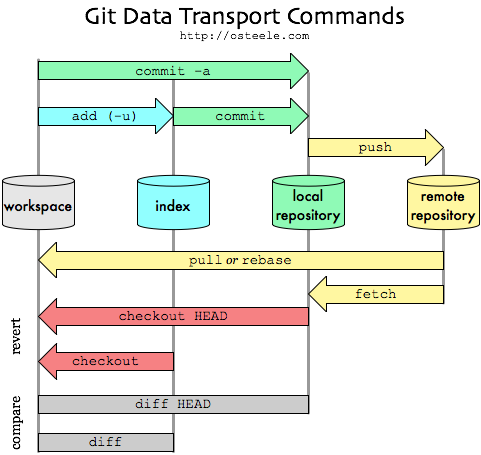
\includegraphics[scale=0.4]{git-transport}
	\end{figure}
\end{frame}

% -----------------------------------------------------------------------------

\begin{frame}[fragile]
	\frametitle{Pushing the changes to the remote repository}
	
	\begin{block}{Local vs. remote changes}
	\texttt{commit} only saves changes \alert{locally}! We need to use \texttt{push} to, well, push the changes to the remote repository. 
	\end{block}
	
	\begin{minted}{console}
	> git push origin master
	\end{minted}
	
\end{frame}

% -----------------------------------------------------------------------------


\begin{frame}[fragile]
	\frametitle{Getting changes from the remote repository}
	
	Getting changes is a two-step process:
	\begin{enumerate}
		\item \texttt{fetch} the changes from the remote repository
		\item \texttt{merge} the changes into your working tree
	\end{enumerate}
	
	\begin{minted}{console}
	> git fetch
	> git status
	> git diff master origin/master
	> git merge origin/master
	\end{minted}
	
	\begin{block}{\texttt{fetch}+\texttt{merge}=\texttt{pull}?}
	\texttt{pull} will do \texttt{fetch} and \texttt{merge} in a single step. However, if \texttt{origin} has changed, you might get yourself into trouble.\footnote{A really nice article advocating the use of \texttt{fetch}+\texttt{merge} can be found on \href{http://longair.net/blog/2009/04/16/git-fetch-and-merge/}{Mark's Blog}} 
	\end{block}
\end{frame}

% -----------------------------------------------------------------------------

\begin{frame}[fragile]
	\frametitle{Discarding unwanted changes}
	
	\begin{block}{Task}
	Make a change to your file. Do not commit.	
	\end{block}
	
	Uncommitted changes can be reverted with \texttt{checkout}:
	\begin{minted}{console}
	> git checkout <yournickname>.md
	\end{minted}
	
	You can also revert to a previous version of a file (an earlier commit)\footnote{now you should start seeing why commit messages are important}:
	\begin{minted}{console}
	> git log --oneline
	> git checkout <commit> <file>
	\end{minted}
	This is the same as making any other change to a file, i.e., it can be committed and pushed.
	% TODO: find out how to discard the change that has been made by the checkout
\end{frame}

% -----------------------------------------------------------------------------

\begin{frame}[fragile]
	\frametitle{Dealing with conflicts (1)}
	
	\begin{block}{Task}
	Work in pairs. Both persons make a change to the same file. One commits and pushes. The other one commits and tries push but fails. He/she needs to fetch + merge first.	
	\end{block}
	
	At other person (not pushed), push fails:
	\begin{minted}{console}
	> git push origin master
	> git fetch
	> git diff master..origin/master
	\end{minted}
	
	\begin{block}{Understanding \texttt{diff}}
	\texttt{git diff a b} shows changes that need to be applied to \texttt{a} to make it the same as \texttt{b}.
	\end{block}
\end{frame}

% -----------------------------------------------------------------------------
\begin{frame}[fragile]
	\frametitle{Dealing with conflicts (2)}
	
	After merging, the file ends up in a conflicted state:
	\begin{minted}{console}
	> git merge origin/master -m "Descriptive message"
	> less <conflicted file>	
	\end{minted}	
	
	Conflict markers inside the file:
	\begin{minted}{console}
	<<<<<<< HEAD
	Code on working branch before the merge
	=======
	Code introduced by the merge
	>>>>>>> origin/master
	\end{minted}

	To resolve the conflict, manually edit the file, mark resolution by \texttt{git add} commit and push:
	\begin{minted}{console}
	> git commit -am "Resolved conflict..."
	> git push origin master
	\end{minted}
	
\end{frame}

% -----------------------------------------------------------------------------



\begin{frame}[fragile]
	\frametitle{Manipulating files}
	
	Newly created files have to be added to git explicitly:
	\begin{minted}{console}
	> mkdir <myname>
	> echo blabla > <myname>/newfile.md
	> git add <myname>/newfile.md
	\end{minted}
	
	When moving files, you have to tell git about it:
	\begin{minted}{console}
	> git mv <myname>.md <myname>
	> git commit -am "Added, moved..."	
	\end{minted}
	
	Same goes for deleting files:
	\begin{minted}{console}
	> git rm myname/myname.md
	> git commit -am "Removed..."
	\end{minted}
	
	\begin{minted}{console}
	
	\end{minted}
	
\end{frame}

% -----------------------------------------------------------------------------

\begin{frame}[fragile]
	\frametitle{Handling binary files}
	
	\begin{block}{Difference between text and binary files}
	Changes to text files are stored incrementally, as diffs, which is very space-efficient. For every change in a binary file, the whole file is stored again. The change persists, even after the file is removed!
	\end{block}
	
	\begin{block}{How to handle binary files}
	Storing binary files is ok if they are small and change infrequently. Otherwise, create a README file with instructions for downloading the files (or a download script, if you want to be fancy).
	\end{block}
	
	\begin{block}{Build output}
	\alert{Never} commit build output (even if it is text, e.g. documentation)!
	\end{block}
\end{frame}

% =============================================================================

\section{Working with branches}

\begin{frame}

\frametitle{Branches in git}
	
\begin{enumerate}
	\item Branches are used to develop features in isolation from each other
	\item Git is specifically designed for efficient work with branches
	\item A branch is simply a pointer to a commit
	\item The default branch name is \alert{master}
\end{enumerate}	
		
\end{frame}

% -----------------------------------------------------------------------------

\begin{frame}[fragile]
	
\frametitle{Creating a branch}
	
\begin{block}{When do I need a branch?}
Generally, every time you start working on a new feature, or any significant change to your code.
\end{block}
	
Creating a branch:
\begin{minted}{console}
> git branch <branch name>
> git status
\end{minted}
	
Listing local branches:
\begin{minted}{console}
> git branch -v
\end{minted}	
	
Switching between branches:
\begin{minted}{console}
> git checkout <branch name>
\end{minted}
	
% TODO: add figures!
	
\end{frame}

% -----------------------------------------------------------------------------

\begin{frame}[fragile]

\frametitle{Working on a branch}
	
Switching back and forth between branches changes the files on your disk!

\begin{block}{Task: Bugfix on a local branch}
There is a bug in the \texttt{fact} function of the demo shell program. Create a new branch (give it a descriptive name) and check it out. Fix the bug. Commit.
\end{block}	

By default, branches are visible only locally. To make them visible at the origin, they must be pushed:
\begin{minted}{console}
> git push -u origin <branch name>
\end{minted}

\begin{block}{Task: New feature on a remote branch}
Implement a \texttt{square} command for the demo shell program, which computes the square of the provided argument. Create a new branch and check it out. Implement the feature. Commit. Push the branch to origin.
\end{block}	

\end{frame}

% -----------------------------------------------------------------------------

\begin{frame}[fragile]

\frametitle{Merging branches locally}

After you are finished working on the bugfix, it's time to merge it back into the master branch.
\begin{minted}{console}
> git checkout master
> git merge <branch name>
\end{minted}

After you are done with the bugfix branch, clean up after yourself by deleting it.
\begin{minted}{console}
> git branch -d <branch name>
\end{minted}
	
Merge conflicts are handled in the same way as discussed before. Remote branches at origin are also just branches, so we have been working with branches all along :) 

\end{frame}

% -----------------------------------------------------------------------------

\begin{frame}[fragile]
	
\frametitle{Pull requests}
	
\begin{block}{Task: Pull request}
Look for your branch in the web interface of the GitHub repo. Create a pull request for your branch. Have your partner review and merge the pull request. Delete the branch after it has been merged.
\end{block}	

\begin{block}{Code review}

Pull requests are an efficient and transparent code review mechanism. Code review is good. Pull requests are good. Use pull requests :)
\end{block}

\end{frame}

% -----------------------------------------------------------------------------

\begin{frame}[fragile]
	
\frametitle{Working with multiple remotes}
	
\begin{block}{Why would I need multiple remotes?}
We can get code changes from any repo, not just the one we originally cloned (which is called \texttt{origin}). A typical example is getting changes from the \texttt{upstream} repo, i.e., the repo that we forked.
\end{block}	

Listing and adding remotes:
\begin{minted}{console}
> git remote add <alias> git@<hostname>:<path to repo>	
> git remote -v	
\end{minted}
	
We can now work with the new remote in the same way as with origin (except for pushing!), e.g.:
\begin{minted}{console}
> git fetch <alias>
> git merge <alias>/<branch>
\end{minted}
	
\end{frame}

% -----------------------------------------------------------------------------

\begin{frame}

\frametitle{Merging upstream changes}

\begin{block}{Task: Merge upstream changes}
Create a remote called \texttt{upstream} pointing to \href{https://github.com/larics/git-tutorial-code.git}{the original repo you forked}. \texttt{fetch} the \texttt{upstream} repo and compare its \texttt{master} branch with your \texttt{master} branch. Merge the \texttt{upstream} \texttt{master} into your \texttt{master}.
\end{block}

\end{frame}

% -----------------------------------------------------------------------------


% =============================================================================

\section{Where to go from here?}

\begin{frame}[fragile]

\frametitle{Tips, further reading and useful links}

	\begin{itemize}	
	\item Install zsh and \href{http://ohmyz.sh/}{oh-my-zsh}, which provide awesome tab completion for git (branch names, commit IDs, git command options...)
	\item When you have mastered the merge workflow from this presentation, read up on the rebase workflow described at the \href{http://larics.fer.hr/farm/laricswiki/doku.php?id=software:git}{LARICS git tutorial}, which enables you to produce much cleaner and linear commit history with fewer merges
	\end{itemize}
	
Some additional literature:
	\begin{itemize}
	\item Every git command supports the \texttt{--help} option, e.g.,
	\begin{minted}{console}
> git help
> git branch --help
	\end{minted}
	\item \href{http://stackoverflow.com/questions/tagged/git}{Stackoverflow} :)
	\item \href{https://git-scm.com/book/en/v2}{The Pro Git book} (The git reference)
	\item \href{http://rogerdudler.github.io/git-guide/}{git - the simple guide} (sort of an online cheatsheet)
	\item \href{http://www-cs-students.stanford.edu/~blynn/gitmagic/}{Git Magic} (tutorial) 
	\item \href{http://www.gitguys.com/}{Git Guys} (tutorial)
	\end{itemize}
	
\end{frame}

% ----------------------------------------------------------------

\begin{frame}
	\frametitle{Some other topics to think about}
	
	\begin{itemize}
		\item Using git on Windows
		\item Setting up access to local git repos for other developers
		\item git submodules
	\end{itemize}

	If you have any questions, feel free to send an email to 
	\href{mailto:damjan.miklic@fer.hr}{damjan.miklic@fer.hr} or
	\href{mailto:juraj.orsulic@fer.hr}{juraj.orsulic@fer.hr}, or visit us in C-XI-16!
	
\end{frame}

% ================================================================

\end{document}
